\documentclass{article}
\usepackage{arxiv}

\usepackage[T2A]{fontenc}			
\usepackage[utf8]{inputenc}			
\usepackage[english,russian]{babel}	
\usepackage{amsmath,amsfonts,amssymb,amsthm,mathrsfs,mathtools} 
\usepackage{url}
\usepackage{booktabs}
\usepackage{nicefrac}
\usepackage{microtype}
\usepackage{lipsum}
\usepackage{graphicx}
\usepackage{natbib}
\usepackage{doi}



\title{Погружение временных рядов с высокой волатильностью в метрическое пространство}

\author{ Эйнуллаев Алтай \\
	Кафедра интеллектуальных систем\\
	Московский физико-технический институт\\
	Долгопрудный \\
	\texttt{einullaev.ae@phystech.edu} \\
	%% examples of more authors
	\And
	Яковлев Константин \\
	Кафедра интеллектуальных систем\\
	Московский физико-технический институт\\
	Долгопрудный \\
	\texttt{iakovlev.kd@phystech.edu} \\
	%% \AND
	%% Coauthor \\
	%% Affiliation \\
	%% Address \\
	%% \texttt{email} \\
	%% \And
	%% Coauthor \\
	%% Affiliation \\
	%% Address \\
	%% \texttt{email} \\
	%% \And
	%% Coauthor \\
	%% Affiliation \\
	%% Address \\
	%% \texttt{email} \\
}
\date{}

\renewcommand{\shorttitle}{\textit{arXiv} Template}

%%% Add PDF metadata to help others organize their library
%%% Once the PDF is generated, you can check the metadata with
%%% $ pdfinfo template.pdf
\hypersetup{
pdftitle={A template for the arxiv style},
pdfsubject={q-bio.NC, q-bio.QM},
pdfauthor={David S.~Hippocampus, Elias D.~Striatum},
pdfkeywords={First keyword, Second keyword, More},
}

\begin{document}
\maketitle

\begin{abstract}
	Рассматривается задача прогнозирования финансовых временных рядов. Основными особенностями таких временных рядов являются высокая волатильность и высокая попарная ковариация. Классическим подходом к решению задачи является выполнение прогноза в исходном пространстве. Новый метод заключается в переходе в пространство попарных расстояний между временными рядами, осуществлении прогноза в нем и переходе обратно в исходное пространство. Для его реализации необходимо ввести функцию расстояния между временными рядами, которая должна удовлетворять определенным свойствам. В данной статье изучаются  эти свойства и проводятся сравнения различных метрик на основе численных экспериментов.

\end{abstract}


\keywords{Временные ряды \and Метрика \and Ковариация}

\section{Introduction}

В текущей статье исследуется задача погружения временных рядов в метрическое пространство. Набору временных рядов ставится в соответствие матрица попарных расстояний и появляется возможность перейти от прогнозирования набора временных рядов к прогнозированию матрицы попарных расстояний. При этом выбор функции расстояния осуществляется так, чтобы по полученной матрице расстояний можно было восстановить прогноз для набора временных рядов.

В статистике, обработке сигналов и многих других областях под временным рядом понимаются последовательно измеренные через некоторые (зачастую равные) промежутки времени данные. \cite{shumway2000time} Прогнозирование временных рядов заключается в построении модели для предсказания будущих событий основываясь на известных событиях прошлого, предсказания будущих данных до того как они будут измерены.

Одними из хорошо известных, классических методов прогнозирования временных рядов являются экспоненциальное сглаживание (англ. Exponential Smoothing) \cite{ES}, LSTM (англ. Long Short-Term Memory) \cite{LSTM}, ARIMA  (англ. autoregressive integrated moving average) \cite{ARIMA}. Главным отличием исследуемого метода от вышеперечисленных является то, что временные ряды прогнозируются при помощи прогнозирования матрицы попарных расстояний.

В качестве простейшей метрики рассматривается ковариация между временными рядами. \cite{Boyd} Таким образом, для набора временных рядов получаем матрицу ковариации. Стоит заметить, что матрица ковариации (матрица попарных расстояний) вычисляется в каждый момент времени. Альтернативные варианты метрики выбираются из класса ядер \cite{shawe2004kernel}.

Численные эксперименты проводятся на трех видах данных: синтетические, сигналы коры головного мозга, финансовые временные ряды. Эксперимент состоит из выполнения прогноза временного ряда при помощи прогнозирования матрицы попарных расстояний. В качестве прогностической модели выбирается линейная регрессия с использованием SSA (англ. Singular Spectrum Analysis) \cite{vautard1992singular}. По результатам экспериментов проводится анализ точности прогноза и его устойчивости в зависимости от выбранной метрики и вида данных. Цель эксперимента состоит в оптимальном выборе функции попарных расстояний для выполнения прогноза.

\section{Problem statement}

Пусть \text{X} $ = \{\mathbf{x} = [x_1, \ldots, x_\text{m}]^T | x_i \in R\}$ --- множество временных рядов, заданных своей реализацией. Обозначим через  $\mathbf{Y} \in R^{n \times m}$ заданный набор из $n$ временных рядов:

\begin{equation}
    \mathbf{Y} = [\mathbf{x}^{(1)}, \ldots, \mathbf{x}^{(n)}]^T.
\end{equation}

 Через $\mathbf{Y}_t \in R^{n \times t}$ обозначим $t < m$ первых столбцов $\mathbf{Y}$: 
 
 \begin{equation}
    \mathbf{Y}_t = [\mathbf{x}_{1:t}^{(1)}, \ldots, \mathbf{x}_{1:t}^{(n)}]^T.
\end{equation}. 

Определим функцию расстояния между временными рядами: $d : \text{X} \times \text{X} \rightarrow R$, удовлетворяющую условиям Мерсера \cite{ghojogh2021reproducing}:

1. $d(\mathbf{x}^{(1)}, \mathbf{x}^{(2)}) = d(\mathbf{x}^{(2)}, \mathbf{x}^{(1)})$ $\forall \mathbf{x}^{(1)}, \mathbf{x}^{(2)} \in \text{X}$.

2. $\forall n \in N$, $\forall \mathbf{x}^{(1)}, \ldots, \mathbf{x}^{(n)} \in X$ матрица $\Sigma \in S_n$, составленная из попарных расстояний между элементами, является неотрицательно определенной.

Обозначим расстояние между временными рядами $\mathbf{x}^{(i)} = [x_1^{(i)}, \ldots, x_t^{(i)}], \mathbf{x}^{(j)} = [x^{(j)}_1, \ldots, x^{(j)}_t]$ следующим образом:

\begin{equation}
    d_t(\mathbf{x}^{(i)}, \mathbf{x}^{(j)}) = d_t(i, j)
\end{equation}

Таким образом, в каждый момент времени $t$ набору временных рядов $\mathbf{Y}_t$ поставлена в соответствие матрица попарных расстояний $\Sigma_t \in \mathcal{S}_n^+$ (симметричная, неотрицательно определенная матрица):

\begin{equation}
    \mathbf{Y}_t \Rightarrow \Sigma_t = \left(
\begin{array}{cccc}
d_t(\mathbf{x}^{(1)}, \mathbf{x}^{(1)}) & d_t(\mathbf{x}^{(1)}, \mathbf{x}^{(2)}) & \ldots & d_t(\mathbf{x}^{(1)}, \mathbf{x}^{(n)})\\
d_t(\mathbf{x}^{(2)}, \mathbf{x}^{(1)}) & d_t(\mathbf{x}^{(2)}, \mathbf{x}^{(2)}) & \ldots & d_t(\mathbf{x}^{(2)}, \mathbf{x}^{(n)})\\
\vdots & \vdots & \ddots & \vdots\\
d_t(\mathbf{x}^{(n)}, \mathbf{x}^{(1)}) & d_t(\mathbf{x}^{(n)}, \mathbf{x}^{(2)}) & \ldots & d_t(\mathbf{x}^{(n)}, \mathbf{x}^{(n)})\\
\end{array}
\right)
\end{equation}

Дадим описание двум используемым прогностическим моделям.

\subsection{Авторегрессия}

Пусть имеем реализацию матрицы попарных расстояний из \text{m} компонент: $\Sigma = [\Sigma_1, \Sigma_2, \ldots, \Sigma_\text{m}]$. Пусть $\Sigma_{\text{m} + 1}$ - прогнозируемая матрица. Авторегрессионная модель:

\begin{equation}
    \hat{\Sigma}_{\text{m} + 1} = \sum\limits_{i = 1}^m a_i\Sigma_{i} + \epsilon_{\text{m} + 1}
\end{equation}

где $a_1, \ldots, a_\text{m} \in R$ --- параметры модели (коэффициенты авторегрессии), $\epsilon_{\text{m} + 1} \in R^{\text{m} \times \text{m}}$ --- белый шум. Обозначим через $mathbf{a} \in R^{\text{m}}$ вектор составленный из параметров модели. Вектор оптимальных параметров модели $\hat{\mathbf{a}} \in R^{\text{m}}$ определяется с помощью решения задачи оптимизации:

\begin{equation}
    \hat{\mathbf{a}} = \arg\min\limits_{\mathbf{a} \in R^{m \times m}}\|\Sigma_{\text{m} + 1} - \hat{\Sigma}_{\text{m} + 1}\|_F^2.
\end{equation}

\subsection{Многомерная гусеница (MSSA)}

Пусть имеем реализацию матрицы попарных расстояний из \text{m} компонент: $\Sigma = [\Sigma_1, \Sigma_2, \ldots, \Sigma_\text{m}]$. Определим \textbf{L} - ширина окна, \text{K} $ = \textbf{m} - \text{L} + 1$. В силу того, что матрица симметричная, то для каждой компоненты матрицы попарных расстояний, где $i \leqslant j$, построим матрицу траекторий (матрица Ганкеля):

\begin{equation}
    \mathbf{H}_{ij} = \left(
\begin{array}{cccc}
d_1(\mathbf{x}^{(i)}, \mathbf{x}^{(j)}) & d_2(\mathbf{x}^{(i)}, \mathbf{x}^{(j)}) & \ldots & d_{\text{K}}(\mathbf{x}^{(i)}, \mathbf{x}^{(j)})\\
d_2(\mathbf{x}^{(i)}, \mathbf{x}^{(j)}) & d_3(\mathbf{x}^{(i)}, \mathbf{x}^{(j)}) & \ldots & d_{\text{K} + 1}(\mathbf{x}^{(i)}, \mathbf{x}^{(j)})\\
\vdots & \vdots & \ddots & \vdots\\
d_{\text{L}}(\mathbf{x}^{(i)}, \mathbf{x}^{(j)}) & d_{\text{L} + 1}(\mathbf{x}^{(i)}, \mathbf{x}^{(j)}) & \ldots & d_\text{m}(\mathbf{x}^{(i)}, \mathbf{x}^{(j)})\\
\end{array}
\right).
\end{equation}

Строим блочную матрицу траекторий:

\begin{equation}
    \mathbf{H} = [\mathbf{H}_{11} : \mathbf{H}_{12} : \mathbf{H}_{13} : \mathbf{H}_{1n} : \mathbf{H}_{22} : \ldots : \mathbf{H}_{nn}]
\end{equation}

Сингулярное разложение симметричной, положительно полуопределенной матрицы $\mathbf{H}\mathbf{H}^T = \mathbf{U}\Lambda\mathbf{U}^T$, где $\Lambda$ - диагональная матрица $\text{L} \times \text{L}$ собственных значений $\lambda_1 \geq \ldots \geq \lambda_{\text{L}}$, $\mathbf{U} = [\mathbf{u}_1, \ldots, \mathbf{u}_{\text{L}}]$ - ортогональная матрица собственных векторов матрицы $\mathbf{H}\mathbf{H}^T$. Пусть $d = \max\{i|\lambda_i > 0, i \in \{1, \ldots, \text{L}\}\}$. Тогда исходную матрицу траекторий можно представить в виде:

\begin{equation}
    \mathbf{H} = \sum\limits_{i = 1}^d\sqrt{\lambda_i}\mathbf{u}_i\mathbf{v}_i^T = \mathbf{H}^{(1)} + \ldots + \mathbf{H}^{(d)} = \sum\limits_{i = 1}^r \mathbf{H}^{(i)} + \sum\limits_{i = r + 1}^d \mathbf{H}^{(i)},
\end{equation}

 где $\mathbf{v}_i = \mathbf{H}^T\mathbf{u}_i/\sqrt{\lambda_i}$ $\mathbf{H}_r = \sum\limits_{i = 1}^{r} \mathbf{H}^{(i)}$ --- сигнальные компоненты, а $\mathbf{H} - \mathbf{H}_r$ --- 
шумовые. Полученную матрицу можно представить в виде:

\begin{equation}
    \mathbf{H}_r = [ \widetilde{\mathbf{H}}_{11} : \widetilde{\mathbf{H}}_{12} : \ldots : \widetilde{\mathbf{H}}_{nn}]
\end{equation}

где каждая из матриц $\widetilde{\mathbf{H}}_{ij} \in R^{\text{m} - \text{L} + 1 \times \text{L}}$. Восстановим исходные расстояния с помощью антидиагонального усреднения элементов соответствующих матриц:

\begin{equation}
    \widetilde{d}_t(i, j) = \dfrac{1}{2t - 1} \sum\limits_{k, l: k + l - 1 = t} \widetilde{h}^{(ij)}_{kl}, t \in \{1, \ldots, m\}
\end{equation}

где $\widetilde{h}^{(ij)}_{kl}$ --- элемент на пересечении $k$-ой строки и $l$-го столбца матрицы $\mathbf{H}_{ij}$. Обозначим через $\mathbf{u}^{\triangledown}_j \in R^{\text{L} - 1}$ первые $\text{L - 1}$ компоненты собственного вектора $\mathbf{u}_j$, а $\pi_j \in R$ --- последнюю компоненту вектора $\mathbf{u}_j$, ($j = 1, \ldots, r$). Определим $v^2 = \sum\limits_{j = 1}^r \pi_{j}^2$ и $\mathbf{p} \in R^{\text{L} - 1}$:

\begin{equation}
    \mathbf{p} = \dfrac{1}{1 - v^2} \sum\limits_{j = 1}^r\pi_j\mathbf{u}_j^{\triangledown}.
\end{equation}

При $v^2 < 1$ возможен прогроз:
\begin{equation}
    [\widetilde{d}_{\text{m} + 1}(1, 1), \widetilde{d}_{\text{m} + 1}(1, 2), \ldots, \widetilde{d}_{\text{m} + 1}(n, n)]^T = \mathbf{p}^T\mathbf{Z}
\end{equation}

где $\mathbf{Z} \in R^{(\text{L} - 1) \times (\frac{n(n + 1)}{2})}$, $\mathbf{Z} = [\mathbf{z}^{(11)}, \ldots, \mathbf{z}^{(nn)}]$, $\mathbf{z}^{(ij)} = [\widetilde{d}_{\text{m} - \text{L} + 2}(i, j), \ldots, \widetilde{d}_{\text{m}}(i, j)]^T$. Таким образом, получаем:

\begin{equation}
    \hat{\Sigma}_{\text{m} + 1} = [\widetilde{d}_{\text{m} + 1}(i, j)]_{i, j = 1}^{n}
\end{equation}

где $\widetilde{d}_{\text{m} + 1}(i, j) = \widetilde{d}_{\text{m} + 1}(j, i)$, при $i > j$.

\subsection{Задача прогнозирования набора временных рядов}

В качестве критериев качества прогноза временных рядов используются 

\begin{equation}
    \text{MAPE} = \frac{1}{m}\sum\limits_{i = 1}^{m}\dfrac{|x^{(i)}_t - \hat{x}^{(i)}_t|}{|x^{(i)}_t|},
\end{equation}

\begin{equation}
    \text{MSE} = \frac{1}{m}\sum\limits_{i = 1}^{m}(x^{(i)}_t - \hat{x}^{(i)}_t)^2.
\end{equation}

Также выбираются $p < m$ временных рядов из набора так, чтобы отказ от прогнозирования соответствующих $m - p$ временных рядов существенно повышал качество \text{MAPE}, \text{MSE}. 

\subsection{Выбор функции попарных расстояний}

Пусть $\mathcal{F} = \{d^{(1)}, \ldots, d^{(s)}\}$ --- множество функций попарных расстояний, из которого нужно выбрать оптимальный вариант. Пусть $\hat{\Sigma}(d)$ --- спрогнозированная, а $\Sigma(d)$ --- точная матрица попарных расстояний при использовании $d \in \mathcal{F}$. Тогда оптимальный по точности выбор функции попарных расстояний:

\begin{equation}
    d_{\text{acc}} = \arg\min\limits_{d \in \mathcal{F}} \sigma^2(d) = \arg\min\limits_{d \in \mathcal{F}} \|\hat{\Sigma}(d) - \Sigma(d)\|_{\text{F}}^2.
\end{equation}

Пусть $\widetilde{\mathbf{x}}^{(i)} = \mathbf{x}^{(i)} + \varepsilon_i$, $i = 1, \ldots, n$ --- зашумленный исходный набор временных рядов, где $\varepsilon_i \in R^\text{N}$. Пусть $\widetilde{\sigma}^2(d)$ --- точность прогноза матрицы попарных расстояний зашумленного набора временных рядов при использовании $d \in \mathcal{F}$. Тогда наболее устойчивый выбор функции попарных расстояний:

\begin{equation}
    d_{\text{stable}} = \arg\min\limits_{d \in \text{F}}|\widetilde{\sigma}^2(d) - \sigma^2(d)|
\end{equation}

\section{Computational experiment}

Целью эксперимента является сравнение качества прогнозирования предложенного метода с классическими методами. В качестве базовых данных рассматриваются синтетические данные двух типов: зашумленный синус заданной амплитуды и зашумленная сумма двух синусов заданной амплитуды с различными периодами. Проведем сравнение методов $\text{MSSA}$ и $\text{AR}$ на синтетических данных, не используя для прогнозирования матрицу попарных расстояний. Для этого, разобьем временной ряд на обучающую и тестовую выборку, спрогнозируем тестовую часть и сравним точность прогноза с помощью $\text{MAPE}$ (15) и $\text{MSE}$ (16).

\subsection{MSSA}

Рассматривается набор временных рядов размера 2, состоящий из двух типов синтетических данных, описанных выше. Каждый временной ряд состоит из $n = 1000$ сигналов, разбиение на обучающую и тестовую выборку осуществляется в пропорции $7:3$. Приведем результаты прогнозирования с помощью MSSA и значения критериев качества прогноза каждого ряда на отдельных графиках:

\begin{figure}[!htbp]
\centering
{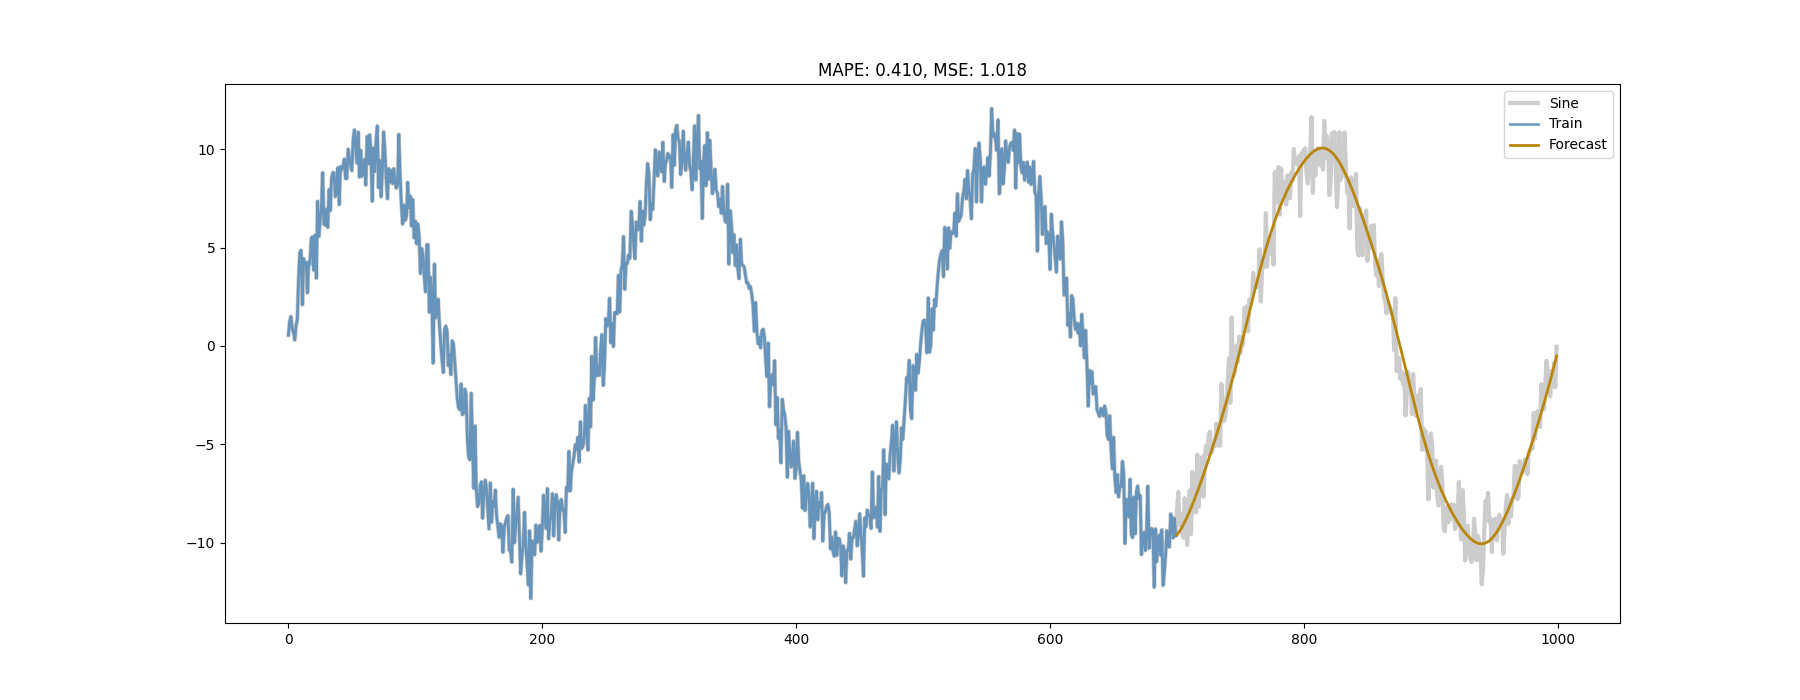
\includegraphics[width=10cm]{images/MSSA_1.png} }
\caption{Прогнозирование зашумленного синуса с помощью MSSA с указанием критериев качества прогноза}
\label{fig:MSSAsine}
\end{figure}

\begin{figure}[!htbp]
\centering
{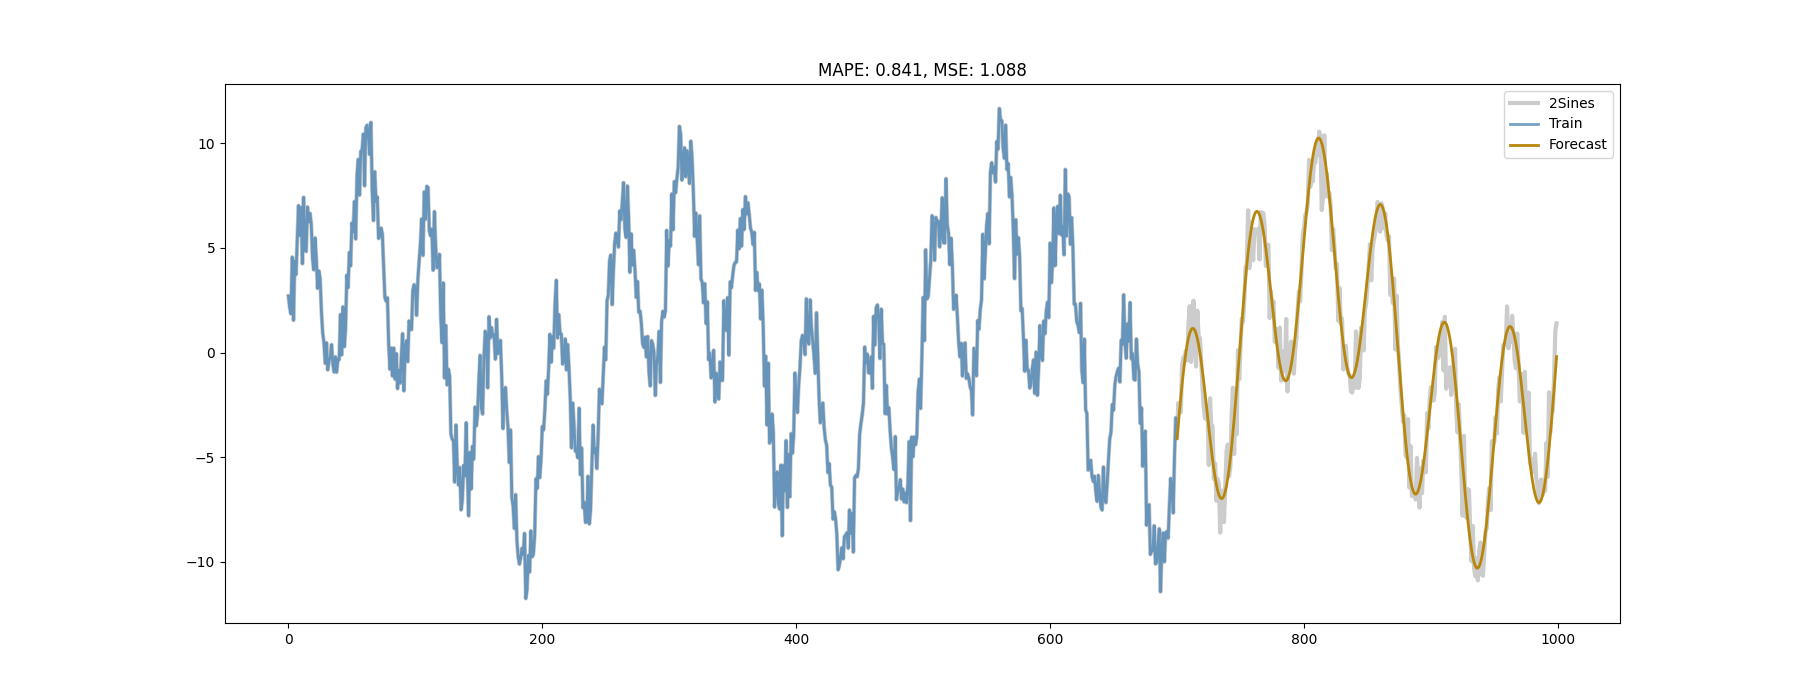
\includegraphics[width=10cm]{images/MSSA_2.png} }
\caption{Прогнозирование зашумленная сумма двух синусов с различными периодами с помощью MSSA с указанием критериев качества прогноза}
\label{fig:MSSA2sines}
\end{figure}

\newpage

\subsection{AR}

В этом случае каждый из временных рядов прогнозировался независимо. Качество прогноза зависит от выбора параметра $p$ --- количество предыдущих значений временного ряда, учавствующих в авторегрессии. В нашем эксперименте $p = 30$. В обоих случаях, при разбиении выборки в пропорциях, использованных в $MSSA$, получали плохое качество прогноза. Поэтому, в обоих случаях, разбиение на обучающую и тестовую выборку осуществляется в пропорции $8:2$. Тем не менее, качество прогноза все равно значительно уступает MSSA, особенно во втором случае.

\begin{figure}[!htbp]
\centering
{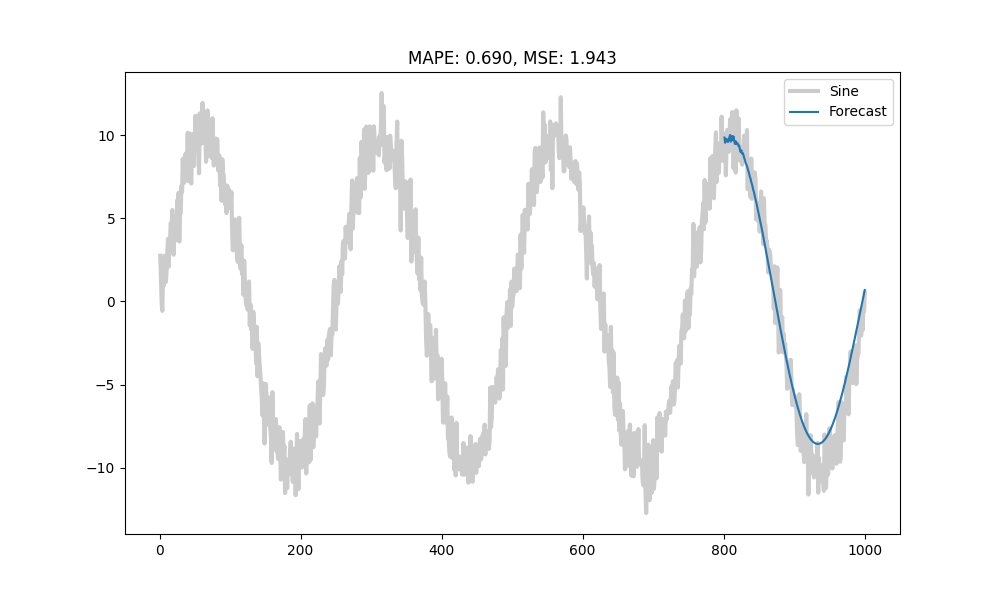
\includegraphics[width=10cm]{images/AR_1.png} }
\caption{Прогнозирование зашумленного синуса с помощью AR с указанием критериев качества прогноза}
\label{fig:ARsine}
\end{figure}

\begin{figure}[!htbp]
\centering
{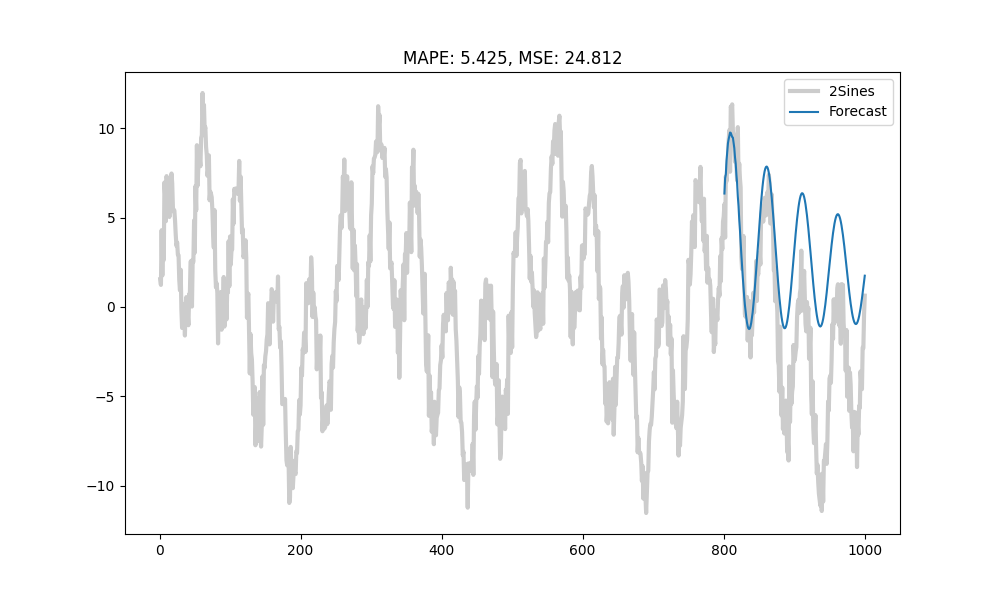
\includegraphics[width=10cm]{images/AR_2.png} }
\caption{Прогнозирование зашумленная сумма двух синусов с различными периодами с помощью AR с указанием критериев качества прогноза}
\label{fig:AR2sines}
\end{figure}

\subsection{LSTM}

В этом случае прогнозировались синтетические и реальные наборы временных рядов с высокой попарной корреляцией. Количество временных рядов в наборе в обоих случаях равно $n = 24$. В качестве синтетических данных снова выступают смещенные относительно друг друга, зашумленные синусы различных амплитуд. В качестве реального датасета --- цены на электричество.

\subsubsection{Синтетические данные}

Приведем матрицу корреляции синтетического набора временных рядов, чтобы убедиться в том, что сделанное выше предположение выполняется:


\begin{figure}[!htbp]
\centering
{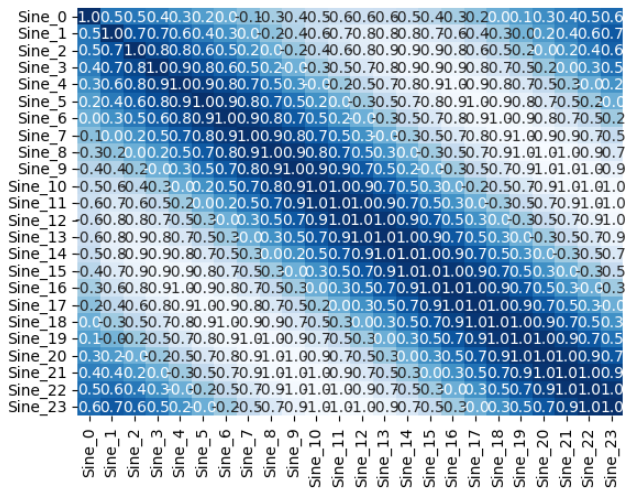
\includegraphics[width=10cm]{images/htmap_sine.png} }
\caption{Матрица корреляции синтетического набора временных рядов}
\label{fig:Heatsine}
\end{figure}

\newpage

 Изобразим на графике результат прогноза двух временных рядов из набора:

\begin{figure}[!htbp]
\centering
{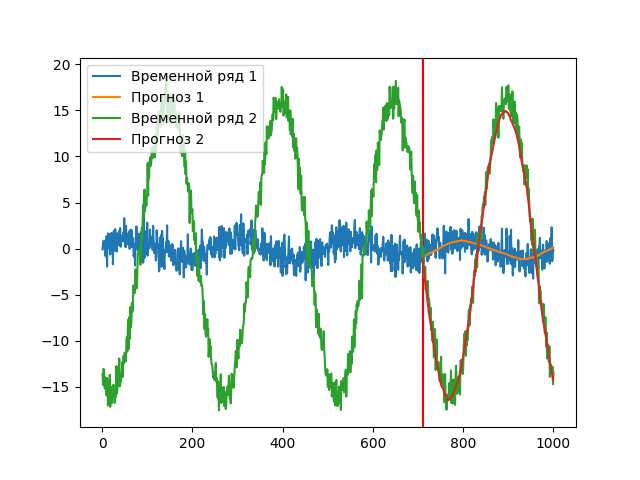
\includegraphics[width=10cm]{images/LSTM_sine.png} }
\caption{Прогнозирование набора зашумленных синусов с помощью LSTM}
\label{fig:LSTMsine}
\end{figure}

Приведем средние ошибки MAPE и MSE прогноза:

\begin{equation}
    \text{MAPE} \approx 0.94
\end{equation}

\begin{equation}
    \text{MSE} \approx 1.36
\end{equation}

\subsubsection{Реальные данные}

Снова приведем матрицу корреляции набора цен на электричество, чтобы убедиться в том, что сделанное выше предположение о высокой попарной корреляции выполняется:

\begin{figure}[!htbp]
\centering
{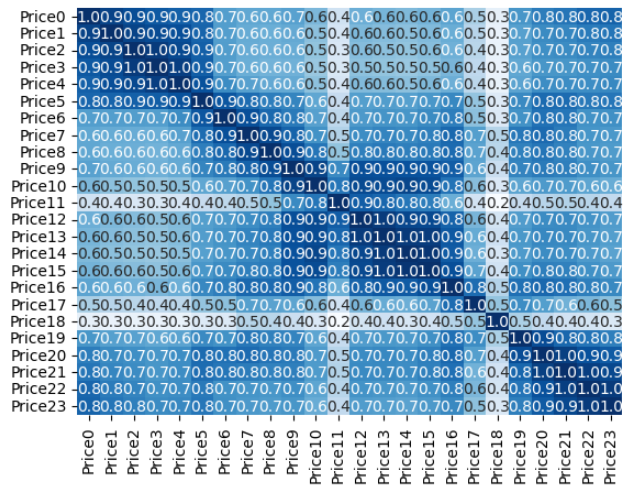
\includegraphics[width=10cm]{images/htmap_price.png} }
\caption{Матрица корреляции набора цен на электричество}
\label{fig:Heatprice}
\end{figure}

 Изобразим на графике результат прогноза двух временных рядов из набора:

\begin{figure}[h]
  \begin{minipage}{0.5\textwidth}
    \centering
    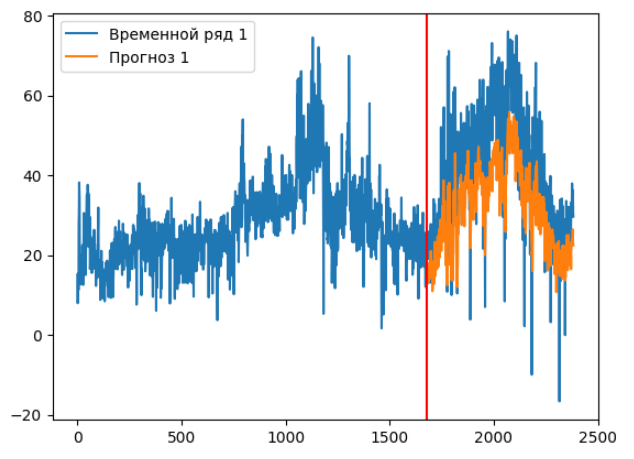
\includegraphics[width=\linewidth]{images/price_1st.png}
  \end{minipage}\hfill
  \begin{minipage}{0.5\textwidth}
    \centering
    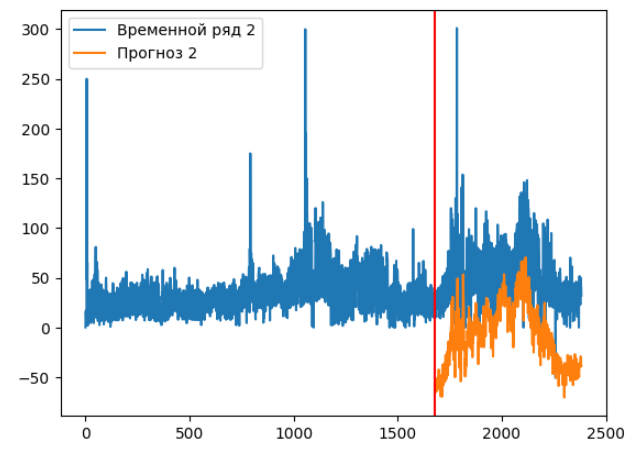
\includegraphics[width=\linewidth]{images/price_2nd.png}
  \end{minipage}
  \caption{Результат прогнозирования на примере двух временных рядов из набора}
\end{figure}

Приведем средние ошибки MAE и MSE прогноза:

\begin{equation}
    \text{MAE} \approx 28.3
\end{equation}

\begin{equation}
    \text{MSE} \approx 1616.6
\end{equation}

Высокая ошибка MSE связана с тем, что в данных, как можно заметить на Pис. 8, имеются очень большие скачки цен. Таким образом, ошибка MAE более информативна.

\bibliographystyle{unsrt}
\bibliography{biblio}

\end{document}
